\iffalse
\let\negmedspace\undefined
\let\negthickspace\undefined
\documentclass[a4,12pt,onecolumn]{IEEEtran}
\usepackage{amsmath,amssymb,amsfonts,amsthm}
\usepackage{algorithmic}
\usepackage{graphicx}
\usepackage{textcomp}
\usepackage{xcolor}
\usepackage{txfonts}
\usepackage{listings}
\usepackage{enumitem}
\usepackage{mathtools}
\usepackage{gensymb}
\usepackage[breaklinks=true]{hyperref}
\usepackage{tkz-euclide}
\usepackage{listings}
\usepackage{circuitikz}
\usepackage{gvv}
\begin{document}
\title{NCERT 12.8 Q4}
\author{EE23BTECH11014 - Devarakonda Guna Vaishnavi $^{}$}
\textbf{Question:} A plane electromagnetic wave travels in vacuum along the \(z\)-direction. What can you say about the directions of its electric (\(\mathbf{E}\)) and magnetic (\(\mathbf{B}\)) field vectors? If the frequency of the wave is \(30 \, \text{MHz}\), what can you say about its wavelength?
 

\solution\\
\fi
\begin{table}[h]
    \centering
    \begin{tabular}{|c|l|c|}
\hline
Symbol & Description                               & Value                    \\ 
\hline
\(c\)    & Speed of light in vacuum                  & \(3 \times 10^8 \, \text{m/s}\) \\
\hline
\(f\)    & Frequency of the electromagnetic wave    & \(30 \, \text{MHz}\)     \\
\hline
\(\lambda\) & Wavelength of the electromagnetic wave   & ?                        \\ \hline
\end{tabular}
    \caption{Input Parameters}
\end{table}

\begin{figure}[h!]
	\centering
	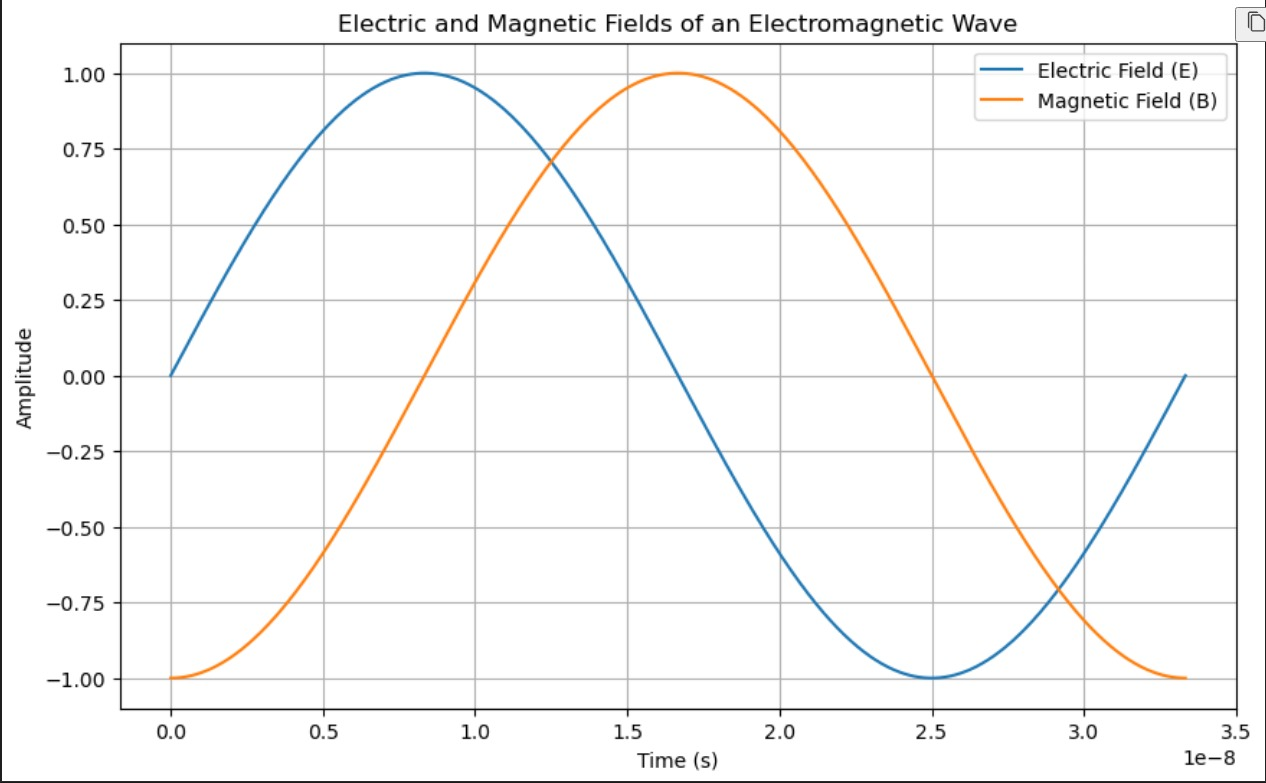
\includegraphics[width=\columnwidth]{ figs/emplot.jpeg}
\end{figure}
 a) A plane electromagnetic wave travels in vacuum along the \(z\)-direction. The electric (\(\mathbf{E}\)) and magnetic (\(\mathbf{B}\)) field vectors are perpendicular to each other move in x and y direction respectively and they are perpendicular to each other
 \vspace{0.2cm}

 b)The relationship between frequency (\(f\)), wavelength (\(\lambda\)), and the speed of light (\(c\)) is given by the formula:
\begin{align}
        \lambda = \frac{c}{f
        \lambda &= \frac{3 \times 10^8 \, \text{m/s}}{30 \times 10^6 \, \text{Hz}} \\
        &= 10 \, \text{m}
 
    
\implies \lambda = 10m  
   \end{align}
